\documentclass[11pt,a4paper]{article}
\usepackage[T1]{fontenc}
\usepackage[utf8]{inputenc}
\usepackage{lmodern}
\usepackage[margin=0.82in]{geometry}
\usepackage{amsmath,amssymb,amsthm,mathtools}
\usepackage{booktabs,array}
\usepackage{caption}
\usepackage{tikz}
\usetikzlibrary{arrows.meta}
\usepackage[hidelinks]{hyperref}
\usepackage{microtype}
\usepackage{enumitem}
\setlength{\parindent}{1.2em}
\setlength{\parskip}{0pt}
\setlist{topsep=3pt,itemsep=1pt}
\newtheorem{theorem}{Theorem}[section]
\newtheorem{proposition}[theorem]{Proposition}
\newtheorem{corollary}[theorem]{Corollary}
\newtheorem{lemma}[theorem]{Lemma}
\theoremstyle{definition}
\newtheorem{definition}[theorem]{Definition}
\newtheorem{example}[theorem]{Example}
\theoremstyle{remark}
\newtheorem{remark}[theorem]{Remark}
\DeclareMathOperator{\ord}{ord}
\DeclareMathOperator{\lcm}{lcm}
\DeclareMathOperator{\gcdop}{gcd}
\title{Orders of Elements in Additive Cyclic Groups:\\[2pt]\large A Least-Common-Multiple Derivation and Residue-Wheel Interpretation}
\author{Md Arif Hossain\\\small Department of Mathematics, Shahjalal University of Science and Technology\\\small Sylhet, Bangladesh}
\date{}
\begin{document}
\maketitle
\begin{abstract}
This paper studies the order of elements in the additive cyclic group $\mathbb Z_n$ through least-common-multiple calculations and residue-wheel diagrams. Repeated addition of a nonzero residue $[a]$ returns to $[0]$ when the cumulative sum first reaches a common multiple of $a$ and $n$, giving $\ord_n([a])=\lcm(a,n)/a=n/\gcd(a,n)$. The wheel representation interprets modular addition as directed jumps around a finite circle and makes the relationship between element order, orbit length, and cycle decomposition explicit. We derive the order formula, establish the corresponding cycle decomposition, examine generators and element-order counts, and compare the algebraic conclusions with a reproducible finite computation.
\end{abstract}
\noindent\textbf{Keywords:} cyclic groups; additive groups; modular arithmetic; element order; greatest common divisor; least common multiple; directed cycles.

\section{Introduction}
The cyclic group of residues modulo a positive integer provides one of the simplest examples of a finite algebraic structure. Its operation is addition modulo $n$, and every element determines a sequence of residues under repeated addition. Finding the first return to zero is exactly the problem of determining the order of that element. This viewpoint offers a direct visual interpretation of the algebraic definition and connects finite group theory with elementary divisibility and algorithms. Standard background on finite groups, modular arithmetic, and elementary number theory can be found in \cite{gallian2021contemporary,finston2014abstract,clapham2014concise,hardy1979introduction}.

Our starting point is the least positive integer that is simultaneously a multiple of the chosen step size $a$ and the modulus $n$. This leads directly to a least-common-multiple expression for the return time under modular addition. Arranging the residue classes on a wheel then turns successive additions into a sequence of directed jumps, making the algebraic calculation visible. We develop the LCM argument first, prove the corresponding order formula, and examine the cyclic structure represented by the wheel diagrams.

\section{Preliminaries}
For an integer $n\ge 1$, write
\[
\mathbb Z_n=\{[0],[1],\ldots,[n-1]\},
\]
where $[a]$ denotes the congruence class of $a$ modulo $n$. Under addition, $\mathbb Z_n$ is a cyclic group with identity $[0]$. As usual, $k[a]$ means the $k$-fold sum $[a]+\cdots+[a]=[ka]$.

\begin{definition}
The \emph{order} of $[a]\in\mathbb Z_n$ is
\[
\ord_n([a])=\min\{k\in\mathbb Z_{>0}:k[a]=[0]\}.
\]
The subgroup generated by $[a]$ is $\langle[a]\rangle=\{k[a]:k\in\mathbb Z\}$.
\end{definition}

\begin{remark}
The identity has order $1$; in particular, $\ord_n([0])=1$. We use the conventions $\gcd(0,n)=n$ and $\lcm(0,n)=0$. Consequently, the quotient $\lcm(a,n)/a$ is stated only for $a\ne0$, whereas the gcd formula also handles $a=0$.
\end{remark}

\subsection*{Residue-wheel viewpoint}
A convenient way to visualize modular addition is to place the classes $[0],[1],\ldots,[n-1]$ evenly around a circle. Starting from $[0]$, repeated addition of a fixed step $[a]$ means moving around this wheel by jumps of size $a$. The order of $[a]$ is then the number of jumps needed to return to the starting point. This geometric picture is elementary, but it encodes the same information as the algebraic definition.

\begin{figure}[ht]
\centering
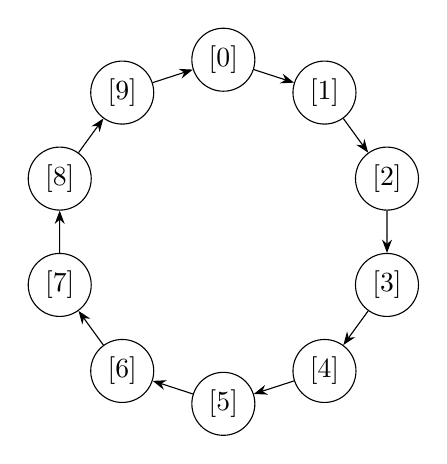
\begin{tikzpicture}[scale=1.15,>=Stealth]
\foreach \k in {0,...,9}{
  \node[draw,circle,inner sep=2.3pt,minimum size=8mm] (z\k) at ({90-36*\k}:1.9cm) {$[\k]$};
}
\foreach \i/\j in {0/1,1/2,2/3,3/4,4/5,5/6,6/7,7/8,8/9,9/0}{
  \draw[->,thin] (z\i) -- (z\j);
}
\end{tikzpicture}
\caption{A residue wheel for $\mathbb Z_{10}$. Arrows indicate the action of adding $[1]$, so one full cycle visits every residue.}
\label{fig:z10wheel}
\end{figure}


\section{From a wheel to the least common multiple}
The motivating question is not initially how to compute a greatest common divisor. It is: \emph{after how many additions of $[a]$ does a walk beginning at $[0]$ return to $[0]$?} For $1\le a<n$, the successive positions are
\[
[0],\ [a],\ [2a],\ldots,[ka],\ldots.
\]
The walk returns to the identity precisely when $ka\equiv0\pmod n$. Equivalently, the positive integer $ka$ must be divisible by $n$. But $ka$ is, by construction, a multiple of $a$. Thus the first return is attained at the \emph{smallest positive common multiple} of $a$ and $n$:
\[
ka=\lcm(a,n),\qquad k=\frac{\lcm(a,n)}{a}.
\]
This is the direct route by which the LCM expression emerges, before introducing the usual gcd expression.

\begin{example}[The first common multiple in $\mathbb Z_{10}$]
Take $a=4$ and $n=10$. Successive positive multiples of $4$ are $4,8,12,16,20,\ldots$, while positive multiples of $10$ are $10,20,30,\ldots$. Their first common term is $20=\lcm(4,10)$. Therefore five additions are required to return to zero:
\[
\ord_{10}([4])=\frac{\lcm(4,10)}{4}=\frac{20}{4}=5.
\]
The corresponding wheel follows $[0]\to[4]\to[8]\to[2]\to[6]\to[0]$, even though the unreduced integer total increases from $0$ to $20$.
\end{example}

\begin{figure}[ht]
\centering
\begin{minipage}[c]{.43\textwidth}
\centering
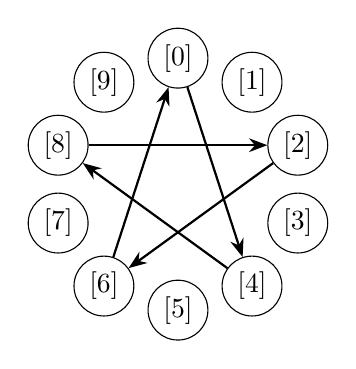
\begin{tikzpicture}[scale=1.0,>=Stealth]
\foreach \k in {0,...,9}{
 \node[draw,circle,inner sep=2pt,minimum size=7.6mm] (w\k) at ({90-36*\k}:1.60cm) {$[\k]$};
}
\foreach \i/\j in {0/4,4/8,8/2,2/6,6/0}{\draw[->,thick] (w\i) -- (w\j);}
\end{tikzpicture}
\end{minipage}\hfill
\begin{minipage}[c]{.51\textwidth}
\centering
\begin{tabular}{@{}rrr@{}}\toprule
Step $k$ & $4k$ & $[4k]_{10}$ \\\midrule
0&0&$[0]$\\
1&4&$[4]$\\
2&8&$[8]$\\
3&12&$[2]$\\
4&16&$[6]$\\
5&20&$[0]$\\\bottomrule
\end{tabular}
\end{minipage}
\caption{The LCM-first residue-wheel construction, illustrated for $[4]\in\mathbb Z_{10}$. The diagram shows the modular positions and the table records the unreduced totals. The first positive multiple of $4$ also divisible by $10$ is $20$, so the first return takes $20/4=5$ jumps.}
\label{fig:lcmwheel}
\end{figure}

\section{The order formula}
\begin{theorem}[LCM-first element-order formula]\label{thm:order}
For every integer $n\ge2$ and $1\le a<n$,
\begin{equation}\label{eq:lcm}
\boxed{\ord_n([a])=\frac{\lcm(a,n)}{a}.}
\end{equation}
Equivalently,
\begin{equation}\label{eq:gcd}
\boxed{\ord_n([a])=\frac{n}{\gcd(a,n)}.}
\end{equation}
For the identity, $\ord_n([0])=1$; the gcd expression continues to hold if $a=0$.
\end{theorem}
\begin{proof}
By definition, $\ord_n([a])$ is the least positive $k$ for which $ka\equiv0\pmod n$. Such a positive integer $ka$ is a common multiple of $a$ and $n$. The least positive common multiple is $L=\lcm(a,n)$. Therefore the smallest possible $k$ is $L/a$, which proves \eqref{eq:lcm}. The standard identity $\gcd(a,n)\lcm(a,n)=an$ yields \eqref{eq:gcd}. Finally, $[0]$ is the identity and has order one, agreeing with $n/\gcd(0,n)=n/n=1$.
\end{proof}

\begin{remark}[A direct gcd proof]
Writing $d=\gcd(a,n)$, $a=da'$, and $n=dn'$ with $\gcd(a',n')=1$ shows that $n\mid ka$ if and only if $n'\mid ka'$, and hence if and only if $n'\mid k$ by Euclid's lemma. Thus the first such $k$ is $n'=n/d$. This gives an equivalent gcd-based expression; the LCM derivation makes the first-return argument particularly transparent.
\end{remark}

\begin{example}[Further first-common-multiple examples]
For $[3]\in\mathbb Z_{10}$, the first shared positive multiple of $3$ and $10$ is $30$, so $\ord_{10}([3])=30/3=10$. For $[6]\in\mathbb Z_9$, the first shared positive multiple is $18$, so $\ord_9([6])=18/6=3$. These give, respectively, a full wheel and three disjoint short cycles when one draws every starting residue.
\end{example}

\begin{example}[The group $\mathbb Z_{10}$]\label{ex:10}
The complete list is shown in Table~\ref{tab:z10}. The wheel model immediately distinguishes different behaviors:
\begin{itemize}
  \item Adding $[1]$ moves to the next residue each time, so every class is visited before returning to $[0]$. Hence $\ord_{10}([1])=10$.
  \item Adding $[2]$ skips every other vertex and therefore traces a 5-cycle through the even residues. Hence $\ord_{10}([2])=5$.
  \item Adding $[4]$ gives
  \[
  [0]\longrightarrow[4]\longrightarrow[8]\longrightarrow[2]\longrightarrow[6]\longrightarrow[0],
  \]
  so $\ord_{10}([4])=5$, agreeing with $10/\gcd(4,10)=5$.
\end{itemize}
\end{example}
\begin{table}[ht]
\centering
\caption{Orders of elements in $\mathbb Z_{10}$}\label{tab:z10}
\begin{tabular}{@{}c*{10}{c}@{}}\toprule
$a$ & 0&1&2&3&4&5&6&7&8&9\\\midrule
$\gcd(a,10)$ &10&1&2&1&2&5&2&1&2&1\\
$\ord_{10}([a])$ &1&10&5&10&5&2&5&10&5&10\\\bottomrule
\end{tabular}
\end{table}

\begin{figure}[ht]
\centering
\begin{minipage}[t]{0.32\textwidth}
\centering
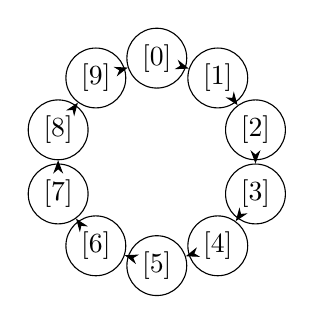
\begin{tikzpicture}[scale=0.85,>=Stealth]
\foreach \k in {0,...,9}{
  \node[draw,circle,inner sep=2.1pt,minimum size=7.6mm] (a\k) at ({90-36*\k}:1.55cm) {$[\k]$};
}
\foreach \i/\j in {0/1,1/2,2/3,3/4,4/5,5/6,6/7,7/8,8/9,9/0}{\draw[->] (a\i) -- (a\j);} 
\end{tikzpicture}
\caption*{(a) Step size $1$}
\end{minipage}\hfill
\begin{minipage}[t]{0.32\textwidth}
\centering
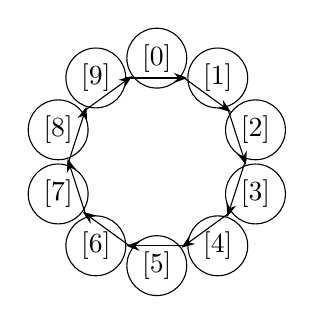
\begin{tikzpicture}[scale=0.85,>=Stealth]
\foreach \k in {0,...,9}{
  \node[draw,circle,inner sep=2.1pt,minimum size=7.6mm] (b\k) at ({90-36*\k}:1.55cm) {$[\k]$};
}
\foreach \i/\j in {0/2,2/4,4/6,6/8,8/0,1/3,3/5,5/7,7/9,9/1}{\draw[->] (b\i) -- (b\j);} 
\end{tikzpicture}
\caption*{(b) Step size $2$}
\end{minipage}\hfill
\begin{minipage}[t]{0.32\textwidth}
\centering
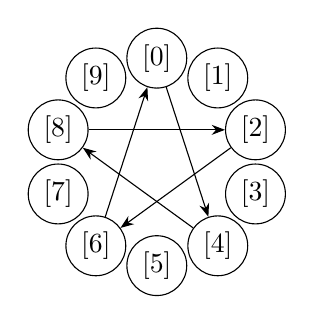
\begin{tikzpicture}[scale=0.85,>=Stealth]
\foreach \k in {0,...,9}{
  \node[draw,circle,inner sep=2.1pt,minimum size=7.6mm] (c\k) at ({90-36*\k}:1.55cm) {$[\k]$};
}
\foreach \i/\j in {0/4,4/8,8/2,2/6,6/0}{\draw[->] (c\i) -- (c\j);} 
\end{tikzpicture}
\caption*{(c) Step size $4$}
\end{minipage}
\caption{Three wheel setups in $\mathbb Z_{10}$. Figure (a) is a single 10-cycle, (b) decomposes into two 5-cycles, and (c) shows the orbit of $[0]$ under repeated addition of $[4]$.}
\label{fig:cycle}
\end{figure}

\section{Residue cycles and generated subgroups}
For a fixed residue $[a]$, define the map $T_a:\mathbb Z_n\to\mathbb Z_n$ by $T_a([r])=[r+a]$. Because addition by $[a]$ is invertible (with inverse addition by $[-a]$), this map is a permutation of the residue classes.

\begin{proposition}[Cycle decomposition]\label{prop:cycles}
If $d=\gcd(a,n)$, the directed graph with vertices $\mathbb Z_n$ and arrows $[r]\to[r+a]$ consists of exactly $d$ disjoint cycles, each of length $n/d$.
\end{proposition}
\begin{proof}
Starting at $[r]$, the successive vertices are $[r+ka]$. The first return to $[r]$ occurs when $ka\equiv0\pmod n$, independently of $r$. By Theorem~\ref{thm:order}, this takes $n/d$ steps. Thus every cycle has length $n/d$. Since there are $n$ vertices in total, the number of cycles is $n/(n/d)=d$.
\end{proof}

\begin{figure}[ht]
\centering
\begin{minipage}[t]{0.47\textwidth}
\centering
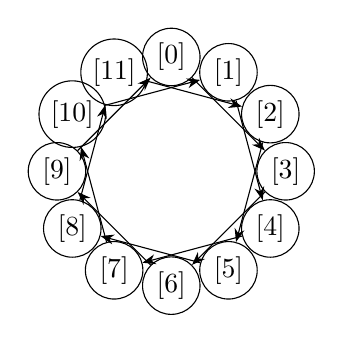
\begin{tikzpicture}[scale=0.88,>=Stealth]
\foreach \k in {0,...,11}{
  \node[draw,circle,inner sep=2pt,minimum size=7.3mm] (u\k) at ({90-30*\k}:1.65cm) {$[\k]$};
}
\foreach \i/\j in {0/3,3/6,6/9,9/0,1/4,4/7,7/10,10/1,2/5,5/8,8/11,11/2}{\draw[->] (u\i) -- (u\j);} 
\end{tikzpicture}
\caption*{(a) Adding $[3]$ in $\mathbb Z_{12}$}
\end{minipage}\hfill
\begin{minipage}[t]{0.47\textwidth}
\centering
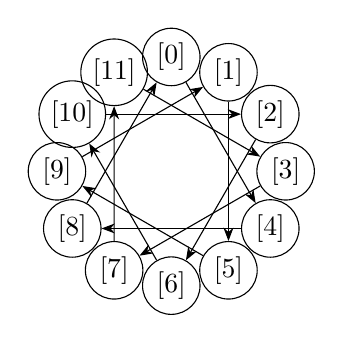
\begin{tikzpicture}[scale=0.88,>=Stealth]
\foreach \k in {0,...,11}{
  \node[draw,circle,inner sep=2pt,minimum size=7.3mm] (v\k) at ({90-30*\k}:1.65cm) {$[\k]$};
}
\foreach \i/\j in {0/4,4/8,8/0,1/5,5/9,9/1,2/6,6/10,10/2,3/7,7/11,11/3}{\draw[->] (v\i) -- (v\j);} 
\end{tikzpicture}
\caption*{(b) Adding $[4]$ in $\mathbb Z_{12}$}
\end{minipage}
\caption{Additional wheel setups in $\mathbb Z_{12}$. In (a), $\gcd(3,12)=3$, so the residues split into three cycles of length $4$. In (b), $\gcd(4,12)=4$, so the residues split into four cycles of length $3$.}
\label{fig:z12wheels}
\end{figure}

\begin{figure}[ht]
\centering
\begin{minipage}[t]{0.47\textwidth}
\centering
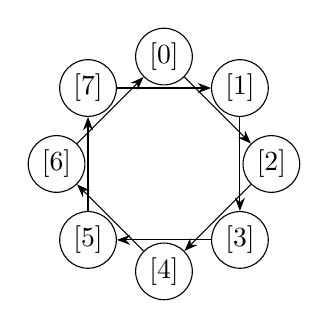
\begin{tikzpicture}[scale=0.88,>=Stealth]
\foreach \k in {0,...,7}{
  \node[draw,circle,inner sep=2pt,minimum size=7.2mm] (p\k) at ({90-45*\k}:1.55cm) {$[\k]$};
}
\foreach \i/\j in {0/2,2/4,4/6,6/0,1/3,3/5,5/7,7/1}{\draw[->] (p\i) -- (p\j);} 
\end{tikzpicture}
\caption*{(a) $\mathbb Z_8$, step size $2$}
\end{minipage}\hfill
\begin{minipage}[t]{0.47\textwidth}
\centering
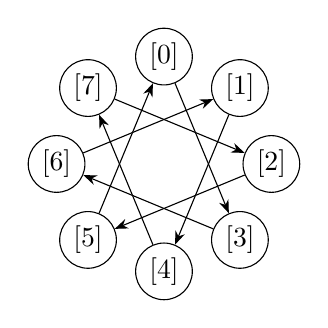
\begin{tikzpicture}[scale=0.88,>=Stealth]
\foreach \k in {0,...,7}{
  \node[draw,circle,inner sep=2pt,minimum size=7.2mm] (q\k) at ({90-45*\k}:1.55cm) {$[\k]$};
}
\foreach \i/\j in {0/3,3/6,6/1,1/4,4/7,7/2,2/5,5/0}{\draw[->] (q\i) -- (q\j);} 
\end{tikzpicture}
\caption*{(b) $\mathbb Z_8$, step size $3$}
\end{minipage}
\caption{Two contrasting wheel setups in $\mathbb Z_8$. In (a), $\gcd(2,8)=2$, so there are two cycles of length $4$. In (b), $\gcd(3,8)=1$, so the wheel is a single 8-cycle and $[3]$ is a generator.}
\label{fig:z8wheels}
\end{figure}

\begin{figure}[ht]
\centering
\begin{minipage}[t]{0.47\textwidth}
\centering
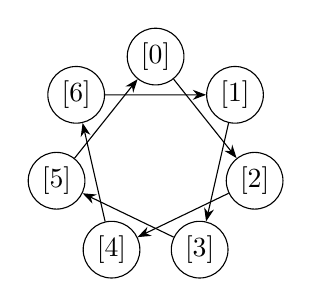
\begin{tikzpicture}[scale=0.86,>=Stealth]
\foreach \k in {0,...,6}{
  \node[draw,circle,inner sep=2pt,minimum size=7.2mm] (r\k) at ({90-360/7*\k}:1.5cm) {$[\k]$};
}
\foreach \i/\j in {0/2,2/4,4/6,6/1,1/3,3/5,5/0}{\draw[->] (r\i) -- (r\j);} 
\end{tikzpicture}
\caption*{(a) $\mathbb Z_7$, step size $2$}
\end{minipage}\hfill
\begin{minipage}[t]{0.47\textwidth}
\centering
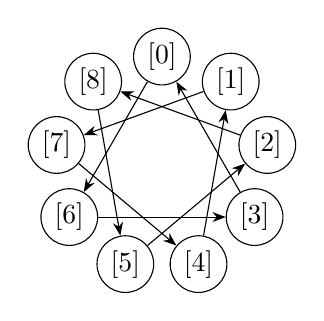
\begin{tikzpicture}[scale=0.86,>=Stealth]
\foreach \k in {0,...,8}{
  \node[draw,circle,inner sep=2pt,minimum size=7.2mm] (s\k) at ({90-40*\k}:1.58cm) {$[\k]$};
}
\foreach \i/\j in {0/6,6/3,3/0,1/7,7/4,4/1,2/8,8/5,5/2}{\draw[->] (s\i) -- (s\j);} 
\end{tikzpicture}
\caption*{(b) $\mathbb Z_9$, step size $6$}
\end{minipage}
\caption{Further wheel setups. In (a), because $7$ is prime and $\gcd(2,7)=1$, the step $[2]$ visits every residue before returning to $[0]$. In (b), $\gcd(6,9)=3$, producing three cycles of length $3$. These examples highlight the contrast between generator and non-generator elements.}
\label{fig:morewheels}
\end{figure}

\begin{corollary}[Subgroup size and generators]\label{cor:generators}
For $[a]\in\mathbb Z_n$,
\[
|\langle[a]\rangle|=\frac{n}{\gcd(a,n)}.
\]
In particular, $[a]$ generates $\mathbb Z_n$ if and only if $\gcd(a,n)=1$.
\end{corollary}
\begin{proof}
The elements of $\langle[a]\rangle$ are exactly the residues visited before the first return to zero. Thus the subgroup has $\ord_n([a])$ elements and has size $n$ precisely when the gcd is $1$.
\end{proof}

\begin{remark}[Prime moduli]
For $n>1$, all nonzero elements of $\mathbb Z_n$ have order $n$ if and only if $n$ is prime. The forward implication follows by choosing a proper nonzero divisor $a$ when $n$ is composite; the reverse implication follows from $\gcd(a,n)=1$ for $1\le a<n$ when $n$ is prime. Thus the order condition provides an equivalent characterization of prime moduli.
\end{remark}

\section{Distribution of element orders}
Let $\varphi$ denote Euler's totient function, with $\varphi(1)=1$.
\begin{proposition}\label{prop:phi}
For every positive divisor $m$ of $n$, the number of elements of order exactly $m$ in $\mathbb Z_n$ is $\varphi(m)$. No other element orders occur.
\end{proposition}
\begin{proof}
By Theorem~\ref{thm:order}, $\ord_n([a])=m$ if and only if $\gcd(a,n)=n/m$. Writing $a=(n/m)t$ with $0\le t<m$, the last condition is equivalent to $\gcd(t,m)=1$. There are $\varphi(m)$ such residues $t$, including the unique case $m=1$ via $t=0$. The same theorem shows that every order divides $n$.
\end{proof}

\begin{example}
For $n=12$, possible orders and their counts are
\[
\begin{array}{c|rrrrrr}
 m&1&2&3&4&6&12\\\hline
 \#\{[a]:\ord_{12}([a])=m\}&1&1&2&2&2&4
\end{array}
\]
The counts sum to $12$, illustrating the classical identity $\sum_{m\mid n}\varphi(m)=n$. The wheel diagrams in Figure~\ref{fig:z12wheels} provide two concrete cases inside this group: the element $[3]$ has order $4$, while $[4]$ has order $3$.
\end{example}

\section{The Chinese remainder viewpoint}
Suppose $n=uv$ with $\gcd(u,v)=1$. The Chinese remainder theorem identifies the additive group $\mathbb Z_n$ with $\mathbb Z_u\times\mathbb Z_v$ under coordinate-wise addition; see \cite{hardy1979introduction}.

\begin{proposition}\label{prop:crt}
If $\gcd(u,v)=1$ and $n=uv$, then
\[
\ord_n([a])=\lcm\!\left(\ord_u([a]),\ord_v([a])\right).
\]
\end{proposition}
\begin{proof}
Under the Chinese remainder isomorphism, $k[a]=[0]$ modulo $n$ holds if and only if $k[a]=[0]$ modulo both $u$ and $v$. The positive integers satisfying these two conditions are the common multiples of the respective coordinate orders; their least positive member is the lcm.
\end{proof}

\begin{example}
Take $n=60=3\cdot4\cdot5$ and $a=9$. The orders of its projections are $\ord_3([0])=1$, $\ord_4([1])=4$, and $\ord_5([4])=5$. Hence $\ord_{60}([9])=\lcm(1,4,5)=20$, in agreement with $60/\gcd(9,60)=20$.
\end{example}

\section{A reproducible computation}
Theorem~\ref{thm:order} can be checked numerically in two independent ways: by calculating a gcd and by repeatedly adding the residue until zero reappears. For each $2\le n\le500$ and each $0\le a<n$, the accompanying Python script computes
\[
\texttt{formula}(a,n)=n/\gcd(a,n)
\]
and compares it with the number of steps in the direct residue walk. The script additionally checks the cycle decomposition described in Proposition~\ref{prop:cycles} and, for each $n$, the predicted number $\varphi(m)$ of elements of every order $m\mid n$.

This finite experiment examines $125{,}249$ element--modulus pairs. All checks pass. The computation provides an independent finite check of the formulas proved above. Whereas direct repeated addition may require as many as $n$ steps, the gcd can be computed efficiently by Euclid's algorithm, with logarithmic arithmetic-operation complexity in the usual classical model.

\section{Discussion and conclusion}
The least-common-multiple viewpoint emphasizes the first positive integer simultaneously divisible by a chosen step size and the modulus. The gcd formula makes the same structure transparent algebraically. Both describe the return time to the identity in an additive cyclic group. The residue-wheel interpretation shows that this return time is also the length of a cycle under modular translation, while $\gcd(a,n)$ counts the number of such cycles. These observations lead directly to generator criteria, the totient distribution of element orders, and the Chinese remainder relation.

The LCM derivation and the residue-wheel representation express the same stopping condition in two forms. In the integer sequence $a,2a,3a,\ldots$, the first return occurs when the accumulated sum equals $\lcm(a,n)$; on the wheel, this is the first directed path that returns to the residue $[0]$. More generally, translation by $[a]$ partitions $\mathbb Z_n$ into exactly $\gcd(a,n)$ disjoint cycles of length $n/\gcd(a,n)$. The wheel diagrams therefore provide a concrete interpretation of element order and subgroup generation, while the divisibility proofs establish these relations for every modulus.

\begin{thebibliography}{9}
\bibitem{clapham2014concise}
Christopher Clapham and James Nicholson.
\emph{The Concise Oxford Dictionary of Mathematics}. 5th ed., Oxford University Press, 2014.
\bibitem{finston2014abstract}
David R. Finston and Patrick J. Morandi.
\emph{Abstract Algebra: Structure and Application}. Birkh\"auser/Springer, 2014. DOI: \href{https://doi.org/10.1007/978-3-319-04498-9}{10.1007/978-3-319-04498-9}.
\bibitem{gallian2021contemporary}
Joseph A. Gallian.
\emph{Contemporary Abstract Algebra}. 10th ed., Chapman and Hall/CRC, 2021.
\bibitem{hardy1979introduction}
G. H. Hardy and E. M. Wright.
\emph{An Introduction to the Theory of Numbers}. 5th ed., Oxford University Press, 1979.
\end{thebibliography}
\end{document}
